\documentclass[1p]{elsarticle_modified}
%\bibliographystyle{elsarticle-num}

%\usepackage[colorlinks]{hyperref}
%\usepackage{abbrmath_seonhwa} %\Abb, \Ascr, \Acal ,\Abf, \Afrak
\usepackage{amsfonts}
\usepackage{amssymb}
\usepackage{amsmath}
\usepackage{amsthm}
\usepackage{scalefnt}
\usepackage{amsbsy}
\usepackage{kotex}
\usepackage{caption}
\usepackage{subfig}
\usepackage{color}
\usepackage{graphicx}
\usepackage{xcolor} %% white, black, red, green, blue, cyan, magenta, yellow
\usepackage{float}
\usepackage{setspace}
\usepackage{hyperref}

\usepackage{tikz}
\usetikzlibrary{arrows}

\usepackage{multirow}
\usepackage{array} % fixed length table
\usepackage{hhline}

%%%%%%%%%%%%%%%%%%%%%
\makeatletter
\renewcommand*\env@matrix[1][\arraystretch]{%
	\edef\arraystretch{#1}%
	\hskip -\arraycolsep
	\let\@ifnextchar\new@ifnextchar
	\array{*\c@MaxMatrixCols c}}
\makeatother %https://tex.stackexchange.com/questions/14071/how-can-i-increase-the-line-spacing-in-a-matrix
%%%%%%%%%%%%%%%

\usepackage[normalem]{ulem}

\newcommand{\msout}[1]{\ifmmode\text{\sout{\ensuremath{#1}}}\else\sout{#1}\fi}
%SOURCE: \msout is \stkout macro in https://tex.stackexchange.com/questions/20609/strikeout-in-math-mode

\newcommand{\cancel}[1]{
	\ifmmode
	{\color{red}\msout{#1}}
	\else
	{\color{red}\sout{#1}}
	\fi
}

\newcommand{\add}[1]{
	{\color{blue}\uwave{#1}}
}

\newcommand{\replace}[2]{
	\ifmmode
	{\color{red}\msout{#1}}{\color{blue}\uwave{#2}}
	\else
	{\color{red}\sout{#1}}{\color{blue}\uwave{#2}}
	\fi
}

\newcommand{\Sol}{\mathcal{S}} %segment
\newcommand{\D}{D} %diagram
\newcommand{\A}{\mathcal{A}} %arc


%%%%%%%%%%%%%%%%%%%%%%%%%%%%%5 test

\def\sl{\operatorname{\textup{SL}}(2,\Cbb)}
\def\psl{\operatorname{\textup{PSL}}(2,\Cbb)}
\def\quan{\mkern 1mu \triangleright \mkern 1mu}

\theoremstyle{definition}
\newtheorem{thm}{Theorem}[section]
\newtheorem{prop}[thm]{Proposition}
\newtheorem{lem}[thm]{Lemma}
\newtheorem{ques}[thm]{Question}
\newtheorem{cor}[thm]{Corollary}
\newtheorem{defn}[thm]{Definition}
\newtheorem{exam}[thm]{Example}
\newtheorem{rmk}[thm]{Remark}
\newtheorem{alg}[thm]{Algorithm}

\newcommand{\I}{\sqrt{-1}}
\begin{document}

%\begin{frontmatter}
%
%\title{Boundary parabolic representations of knots up to 8 crossings}
%
%%% Group authors per affiliation:
%\author{Yunhi Cho} 
%\address{Department of Mathematics, University of Seoul, Seoul, Korea}
%\ead{yhcho@uos.ac.kr}
%
%
%\author{Seonhwa Kim} %\fnref{s_kim}}
%\address{Center for Geometry and Physics, Institute for Basic Science, Pohang, 37673, Korea}
%\ead{ryeona17@ibs.re.kr}
%
%\author{Hyuk Kim}
%\address{Department of Mathematical Sciences, Seoul National University, Seoul 08826, Korea}
%\ead{hyukkim@snu.ac.kr}
%
%\author{Seokbeom Yoon}
%\address{Department of Mathematical Sciences, Seoul National University, Seoul, 08826,  Korea}
%\ead{sbyoon15@snu.ac.kr}
%
%\begin{abstract}
%We find all boundary parabolic representation of knots up to 8 crossings.
%
%\end{abstract}
%\begin{keyword}
%    \MSC[2010] 57M25 
%\end{keyword}
%
%\end{frontmatter}

%\linenumbers
%\tableofcontents
%
\newcommand\colored[1]{\textcolor{white}{\rule[-0.35ex]{0.8em}{1.4ex}}\kern-0.8em\color{red} #1}%
%\newcommand\colored[1]{\textcolor{white}{ #1}\kern-2.17ex	\textcolor{white}{ #1}\kern-1.81ex	\textcolor{white}{ #1}\kern-2.15ex\color{red}#1	}

{\Large $\underline{12a_{1146}~(K12a_{1146})}$}

\setlength{\tabcolsep}{10pt}
\renewcommand{\arraystretch}{1.6}
\vspace{1cm}\begin{tabular}{m{100pt}>{\centering\arraybackslash}m{274pt}}
\multirow{5}{120pt}{
	\centering
	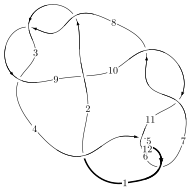
\includegraphics[width=112pt]{../../../GIT/diagram.site/Diagrams/png/1947_12a_1146.png}\\
\ \ \ A knot diagram\footnotemark}&
\allowdisplaybreaks
\textbf{Linearized knot diagam} \\
\cline{2-2}
 &
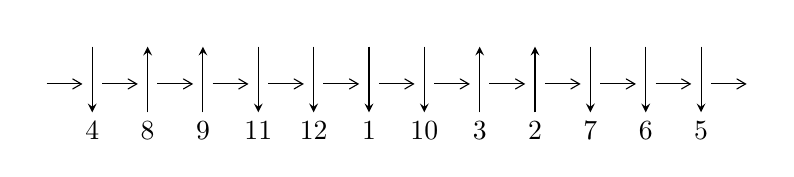
\begin{tikzpicture}[x=20pt, y=17pt]
	% nodes
	\node (C0) at (0, 0) {};
	\node (C1) at (1, 0) {};
	\node (C1U) at (1, +1) {};
	\node (C1D) at (1, -1) {4};

	\node (C2) at (2, 0) {};
	\node (C2U) at (2, +1) {};
	\node (C2D) at (2, -1) {8};

	\node (C3) at (3, 0) {};
	\node (C3U) at (3, +1) {};
	\node (C3D) at (3, -1) {9};

	\node (C4) at (4, 0) {};
	\node (C4U) at (4, +1) {};
	\node (C4D) at (4, -1) {11};

	\node (C5) at (5, 0) {};
	\node (C5U) at (5, +1) {};
	\node (C5D) at (5, -1) {12};

	\node (C6) at (6, 0) {};
	\node (C6U) at (6, +1) {};
	\node (C6D) at (6, -1) {1};

	\node (C7) at (7, 0) {};
	\node (C7U) at (7, +1) {};
	\node (C7D) at (7, -1) {10};

	\node (C8) at (8, 0) {};
	\node (C8U) at (8, +1) {};
	\node (C8D) at (8, -1) {3};

	\node (C9) at (9, 0) {};
	\node (C9U) at (9, +1) {};
	\node (C9D) at (9, -1) {2};

	\node (C10) at (10, 0) {};
	\node (C10U) at (10, +1) {};
	\node (C10D) at (10, -1) {7};

	\node (C11) at (11, 0) {};
	\node (C11U) at (11, +1) {};
	\node (C11D) at (11, -1) {6};

	\node (C12) at (12, 0) {};
	\node (C12U) at (12, +1) {};
	\node (C12D) at (12, -1) {5};
	\node (C13) at (13, 0) {};

	% arrows
	\draw[->,>={angle 60}]
	(C0) edge (C1) (C1) edge (C2) (C2) edge (C3) (C3) edge (C4) (C4) edge (C5) (C5) edge (C6) (C6) edge (C7) (C7) edge (C8) (C8) edge (C9) (C9) edge (C10) (C10) edge (C11) (C11) edge (C12) (C12) edge (C13) ;	\draw[->,>=stealth]
	(C1U) edge (C1D) (C2D) edge (C2U) (C3D) edge (C3U) (C4U) edge (C4D) (C5U) edge (C5D) (C6U) edge (C6D) (C7U) edge (C7D) (C8D) edge (C8U) (C9D) edge (C9U) (C10U) edge (C10D) (C11U) edge (C11D) (C12U) edge (C12D) ;
	\end{tikzpicture} \\
\hhline{~~} \\& 
\textbf{Solving Sequence} \\ \cline{2-2} 
 &
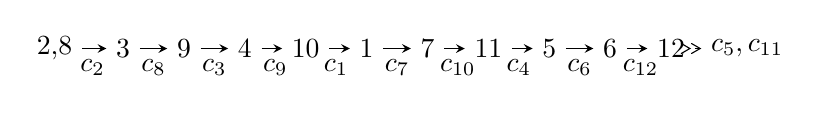
\begin{tikzpicture}[x=22pt, y=7pt]
	% node
	\node (A0) at (-1/8, 0) {2,8};
	\node (A1) at (1, 0) {3};
	\node (A2) at (2, 0) {9};
	\node (A3) at (3, 0) {4};
	\node (A4) at (4, 0) {10};
	\node (A5) at (5, 0) {1};
	\node (A6) at (6, 0) {7};
	\node (A7) at (7, 0) {11};
	\node (A8) at (8, 0) {5};
	\node (A9) at (9, 0) {6};
	\node (A10) at (10, 0) {12};
	\node (C1) at (1/2, -1) {$c_{2}$};
	\node (C2) at (3/2, -1) {$c_{8}$};
	\node (C3) at (5/2, -1) {$c_{3}$};
	\node (C4) at (7/2, -1) {$c_{9}$};
	\node (C5) at (9/2, -1) {$c_{1}$};
	\node (C6) at (11/2, -1) {$c_{7}$};
	\node (C7) at (13/2, -1) {$c_{10}$};
	\node (C8) at (15/2, -1) {$c_{4}$};
	\node (C9) at (17/2, -1) {$c_{6}$};
	\node (C10) at (19/2, -1) {$c_{12}$};
	\node (A11) at (45/4, 0) {$c_{5},c_{11}$};

	% edge
	\draw[->,>=stealth]	
	(A0) edge (A1) (A1) edge (A2) (A2) edge (A3) (A3) edge (A4) (A4) edge (A5) (A5) edge (A6) (A6) edge (A7) (A7) edge (A8) (A8) edge (A9) (A9) edge (A10) ;
	\draw[->>,>={angle 60}]	
	(A10) edge (A11);
\end{tikzpicture} \\ 

\end{tabular} \\

\footnotetext{
The image of knot diagram is generated by the software ``\textbf{Draw programme}" developed by Andrew Bartholomew(\url{http://www.layer8.co.uk/maths/draw/index.htm\#Running-draw}), where we modified some parts for our purpose(\url{https://github.com/CATsTAILs/LinksPainter}).
}\phantom \\ \newline 
\centering \textbf{Ideals for irreducible components\footnotemark of $X_{\text{par}}$} 
 
\begin{align*}
I^u_{1}&=\langle 
u^{58}- u^{57}+\cdots- u+1\rangle \\
\\
\end{align*}
\raggedright * 1 irreducible components of $\dim_{\mathbb{C}}=0$, with total 58 representations.\\
\footnotetext{All coefficients of polynomials are rational numbers. But the coefficients are sometimes approximated in decimal forms when there is not enough margin.}
\newpage
\renewcommand{\arraystretch}{1}
\centering \section*{I. $I^u_{1}= \langle u^{58}- u^{57}+\cdots- u+1 \rangle$}
\flushleft \textbf{(i) Arc colorings}\\
\begin{tabular}{m{7pt} m{180pt} m{7pt} m{180pt} }
\flushright $a_{2}=$&$\begin{pmatrix}1\\0\end{pmatrix}$ \\
\flushright $a_{8}=$&$\begin{pmatrix}0\\u\end{pmatrix}$ \\
\flushright $a_{3}=$&$\begin{pmatrix}1\\- u^2\end{pmatrix}$ \\
\flushright $a_{9}=$&$\begin{pmatrix}u\\- u^3+u\end{pmatrix}$ \\
\flushright $a_{4}=$&$\begin{pmatrix}- u^2+1\\u^4-2 u^2\end{pmatrix}$ \\
\flushright $a_{10}=$&$\begin{pmatrix}- u^3+2 u\\- u^3+u\end{pmatrix}$ \\
\flushright $a_{1}=$&$\begin{pmatrix}u^6-3 u^4+2 u^2+1\\- u^8+4 u^6-4 u^4\end{pmatrix}$ \\
\flushright $a_{7}=$&$\begin{pmatrix}u^7-4 u^5+4 u^3\\u^7-3 u^5+2 u^3+u\end{pmatrix}$ \\
\flushright $a_{11}=$&$\begin{pmatrix}- u^{11}+6 u^9-12 u^7+8 u^5- u^3+2 u\\- u^{11}+5 u^9-8 u^7+3 u^5+u^3+u\end{pmatrix}$ \\
\flushright $a_{5}=$&$\begin{pmatrix}- u^{26}+13 u^{24}+\cdots+u^2+1\\- u^{26}+12 u^{24}+\cdots+6 u^4- u^2\end{pmatrix}$ \\
\flushright $a_{6}=$&$\begin{pmatrix}u^{21}-10 u^{19}+\cdots+10 u^3+u\\- u^{23}+11 u^{21}+\cdots+2 u^3+u\end{pmatrix}$ \\
\flushright $a_{12}=$&$\begin{pmatrix}u^{55}-26 u^{53}+\cdots+10 u^5+2 u\\- u^{57}+27 u^{55}+\cdots+2 u^3+u\end{pmatrix}$\\&\end{tabular}
\flushleft \textbf{(ii) Obstruction class $= -1$}\\~\\
\flushleft \textbf{(iii) Cusp Shapes $= 4 u^{55}-104 u^{53}+\cdots-12 u-2$}\\~\\
\newpage\renewcommand{\arraystretch}{1}
\flushleft \textbf{(iv) u-Polynomials at the component}\newline \\
\begin{tabular}{m{50pt}|m{274pt}}
Crossings & \hspace{64pt}u-Polynomials at each crossing \\
\hline $$\begin{aligned}c_{1},c_{7},c_{10}\end{aligned}$$&$\begin{aligned}
&u^{58}-7 u^{57}+\cdots-79 u+7
\end{aligned}$\\
\hline $$\begin{aligned}c_{2},c_{3},c_{8}\end{aligned}$$&$\begin{aligned}
&u^{58}- u^{57}+\cdots- u+1
\end{aligned}$\\
\hline $$\begin{aligned}c_{4},c_{6}\end{aligned}$$&$\begin{aligned}
&u^{58}- u^{57}+\cdots-3 u+2
\end{aligned}$\\
\hline $$\begin{aligned}c_{5},c_{11},c_{12}\end{aligned}$$&$\begin{aligned}
&u^{58}+u^{57}+\cdots+u+1
\end{aligned}$\\
\hline $$\begin{aligned}c_{9}\end{aligned}$$&$\begin{aligned}
&u^{58}+3 u^{57}+\cdots-129 u-192
\end{aligned}$\\
\hline
\end{tabular}\\~\\
\newpage\renewcommand{\arraystretch}{1}
\flushleft \textbf{(v) Riley Polynomials at the component}\newline \\
\begin{tabular}{m{50pt}|m{274pt}}
Crossings & \hspace{64pt}Riley Polynomials at each crossing \\
\hline $$\begin{aligned}c_{1},c_{7},c_{10}\end{aligned}$$&$\begin{aligned}
&y^{58}+61 y^{57}+\cdots+913 y+49
\end{aligned}$\\
\hline $$\begin{aligned}c_{2},c_{3},c_{8}\end{aligned}$$&$\begin{aligned}
&y^{58}-55 y^{57}+\cdots+5 y+1
\end{aligned}$\\
\hline $$\begin{aligned}c_{4},c_{6}\end{aligned}$$&$\begin{aligned}
&y^{58}-27 y^{57}+\cdots+23 y+4
\end{aligned}$\\
\hline $$\begin{aligned}c_{5},c_{11},c_{12}\end{aligned}$$&$\begin{aligned}
&y^{58}+49 y^{57}+\cdots+5 y+1
\end{aligned}$\\
\hline $$\begin{aligned}c_{9}\end{aligned}$$&$\begin{aligned}
&y^{58}-27 y^{57}+\cdots-1316865 y+36864
\end{aligned}$\\
\hline
\end{tabular}\\~\\
\newpage\flushleft \textbf{(vi) Complex Volumes and Cusp Shapes}
$$\begin{array}{c|c|c}  
\text{Solutions to }I^u_{1}& \I (\text{vol} + \sqrt{-1}CS) & \text{Cusp shape}\\
 \hline 
\begin{aligned}
u &= -1.14724\phantom{ +0.000000I}\end{aligned}
 & -1.35276\phantom{ +0.000000I} & \phantom{-0.000000 } 0 \\ \hline\begin{aligned}
u &= \phantom{-}1.151380 + 0.058161 I\end{aligned}
 & \phantom{-}2.53228 + 3.79612 I & \phantom{-0.000000 } 0 \\ \hline\begin{aligned}
u &= \phantom{-}1.151380 - 0.058161 I\end{aligned}
 & \phantom{-}2.53228 - 3.79612 I & \phantom{-0.000000 } 0 \\ \hline\begin{aligned}
u &= \phantom{-}0.481555 + 0.664903 I\end{aligned}
 & \phantom{-}11.99140 + 2.20783 I & \phantom{-}4.22893 - 3.07025 I \\ \hline\begin{aligned}
u &= \phantom{-}0.481555 - 0.664903 I\end{aligned}
 & \phantom{-}11.99140 - 2.20783 I & \phantom{-}4.22893 + 3.07025 I \\ \hline\begin{aligned}
u &= -0.443054 + 0.686901 I\end{aligned}
 & \phantom{-}7.60131 - 10.06700 I & \phantom{-}0.80807 + 7.84045 I \\ \hline\begin{aligned}
u &= -0.443054 - 0.686901 I\end{aligned}
 & \phantom{-}7.60131 + 10.06700 I & \phantom{-}0.80807 - 7.84045 I \\ \hline\begin{aligned}
u &= -0.515153 + 0.627947 I\end{aligned}
 & \phantom{-}7.87503 + 5.69223 I & \phantom{-}1.58915 - 1.87939 I \\ \hline\begin{aligned}
u &= -0.515153 - 0.627947 I\end{aligned}
 & \phantom{-}7.87503 - 5.69223 I & \phantom{-}1.58915 + 1.87939 I \\ \hline\begin{aligned}
u &= \phantom{-}0.438326 + 0.675169 I\end{aligned}
 & \phantom{-}2.65616 + 6.14445 I & -3.69389 - 6.69694 I \\ \hline\begin{aligned}
u &= \phantom{-}0.438326 - 0.675169 I\end{aligned}
 & \phantom{-}2.65616 - 6.14445 I & -3.69389 + 6.69694 I \\ \hline\begin{aligned}
u &= \phantom{-}0.501005 + 0.618665 I\end{aligned}
 & \phantom{-}2.90568 - 1.85234 I & -2.97160 + 0.63684 I \\ \hline\begin{aligned}
u &= \phantom{-}0.501005 - 0.618665 I\end{aligned}
 & \phantom{-}2.90568 + 1.85234 I & -2.97160 - 0.63684 I \\ \hline\begin{aligned}
u &= -0.442362 + 0.648377 I\end{aligned}
 & \phantom{-}5.01043 - 2.20484 I & -0.34907 + 2.50917 I \\ \hline\begin{aligned}
u &= -0.442362 - 0.648377 I\end{aligned}
 & \phantom{-}5.01043 + 2.20484 I & -0.34907 - 2.50917 I \\ \hline\begin{aligned}
u &= -0.466755 + 0.626215 I\end{aligned}
 & \phantom{-}5.10910 - 1.98014 I & \phantom{-}0.15978 + 4.14976 I \\ \hline\begin{aligned}
u &= -0.466755 - 0.626215 I\end{aligned}
 & \phantom{-}5.10910 + 1.98014 I & \phantom{-}0.15978 - 4.14976 I \\ \hline\begin{aligned}
u &= -1.307560 + 0.189347 I\end{aligned}
 & \phantom{-}4.08058 - 1.65712 I & \phantom{-0.000000 } 0 \\ \hline\begin{aligned}
u &= -1.307560 - 0.189347 I\end{aligned}
 & \phantom{-}4.08058 + 1.65712 I & \phantom{-0.000000 } 0 \\ \hline\begin{aligned}
u &= \phantom{-}1.331250 + 0.207988 I\end{aligned}
 & \phantom{-}0.86765 + 5.45245 I & \phantom{-0.000000 } 0 \\ \hline\begin{aligned}
u &= \phantom{-}1.331250 - 0.207988 I\end{aligned}
 & \phantom{-}0.86765 - 5.45245 I & \phantom{-0.000000 } 0 \\ \hline\begin{aligned}
u &= \phantom{-}0.188380 + 0.617055 I\end{aligned}
 & \phantom{-}0.49984 + 6.30818 I & -4.83696 - 8.02356 I \\ \hline\begin{aligned}
u &= \phantom{-}0.188380 - 0.617055 I\end{aligned}
 & \phantom{-}0.49984 - 6.30818 I & -4.83696 + 8.02356 I \\ \hline\begin{aligned}
u &= \phantom{-}1.354390 + 0.050533 I\end{aligned}
 & \phantom{-}3.56112 + 0.15774 I & \phantom{-0.000000 } 0 \\ \hline\begin{aligned}
u &= \phantom{-}1.354390 - 0.050533 I\end{aligned}
 & \phantom{-}3.56112 - 0.15774 I & \phantom{-0.000000 } 0 \\ \hline\begin{aligned}
u &= -1.351690 + 0.130313 I\end{aligned}
 & \phantom{-}4.61294 - 2.74721 I & \phantom{-0.000000 } 0 \\ \hline\begin{aligned}
u &= -1.351690 - 0.130313 I\end{aligned}
 & \phantom{-}4.61294 + 2.74721 I & \phantom{-0.000000 } 0 \\ \hline\begin{aligned}
u &= -1.345480 + 0.220131 I\end{aligned}
 & \phantom{-}5.32159 - 9.34589 I & \phantom{-0.000000 } 0 \\ \hline\begin{aligned}
u &= -1.345480 - 0.220131 I\end{aligned}
 & \phantom{-}5.32159 + 9.34589 I & \phantom{-0.000000 } 0 \\ \hline\begin{aligned}
u &= -0.155934 + 0.602452 I\end{aligned}
 & -3.78873 - 2.51425 I & -10.60618 + 5.42125 I\\
 \hline 
 \end{array}$$\newpage$$\begin{array}{c|c|c}  
\text{Solutions to }I^u_{1}& \I (\text{vol} + \sqrt{-1}CS) & \text{Cusp shape}\\
 \hline 
\begin{aligned}
u &= -0.155934 - 0.602452 I\end{aligned}
 & -3.78873 + 2.51425 I & -10.60618 - 5.42125 I \\ \hline\begin{aligned}
u &= \phantom{-}0.107983 + 0.596551 I\end{aligned}
 & -0.304445 - 1.182970 I & -7.28418 - 0.76991 I \\ \hline\begin{aligned}
u &= \phantom{-}0.107983 - 0.596551 I\end{aligned}
 & -0.304445 + 1.182970 I & -7.28418 + 0.76991 I \\ \hline\begin{aligned}
u &= -0.366762 + 0.465079 I\end{aligned}
 & \phantom{-}4.44827 - 1.54185 I & \phantom{-}2.24711 + 4.56850 I \\ \hline\begin{aligned}
u &= -0.366762 - 0.465079 I\end{aligned}
 & \phantom{-}4.44827 + 1.54185 I & \phantom{-}2.24711 - 4.56850 I \\ \hline\begin{aligned}
u &= -1.411190 + 0.054492 I\end{aligned}
 & \phantom{-}8.16493 + 2.73473 I & \phantom{-0.000000 } 0 \\ \hline\begin{aligned}
u &= -1.411190 - 0.054492 I\end{aligned}
 & \phantom{-}8.16493 - 2.73473 I & \phantom{-0.000000 } 0 \\ \hline\begin{aligned}
u &= \phantom{-}1.40642 + 0.15083 I\end{aligned}
 & \phantom{-}10.05250 + 3.76035 I & \phantom{-0.000000 } 0 \\ \hline\begin{aligned}
u &= \phantom{-}1.40642 - 0.15083 I\end{aligned}
 & \phantom{-}10.05250 - 3.76035 I & \phantom{-0.000000 } 0 \\ \hline\begin{aligned}
u &= \phantom{-}0.547094 + 0.139034 I\end{aligned}
 & \phantom{-}2.23185 - 3.44215 I & \phantom{-}0.89332 + 2.64024 I \\ \hline\begin{aligned}
u &= \phantom{-}0.547094 - 0.139034 I\end{aligned}
 & \phantom{-}2.23185 + 3.44215 I & \phantom{-}0.89332 - 2.64024 I \\ \hline\begin{aligned}
u &= -0.511205\phantom{ +0.000000I}\end{aligned}
 & -1.78784\phantom{ +0.000000I} & -4.31540\phantom{ +0.000000I} \\ \hline\begin{aligned}
u &= \phantom{-}1.47373 + 0.23609 I\end{aligned}
 & \phantom{-}11.19640 + 5.44235 I & \phantom{-0.000000 } 0 \\ \hline\begin{aligned}
u &= \phantom{-}1.47373 - 0.23609 I\end{aligned}
 & \phantom{-}11.19640 - 5.44235 I & \phantom{-0.000000 } 0 \\ \hline\begin{aligned}
u &= \phantom{-}1.47805 + 0.22330 I\end{aligned}
 & \phantom{-}11.39260 + 5.08524 I & \phantom{-0.000000 } 0 \\ \hline\begin{aligned}
u &= \phantom{-}1.47805 - 0.22330 I\end{aligned}
 & \phantom{-}11.39260 - 5.08524 I & \phantom{-0.000000 } 0 \\ \hline\begin{aligned}
u &= -1.47640 + 0.24549 I\end{aligned}
 & \phantom{-}8.84229 - 9.50759 I & \phantom{-0.000000 } 0 \\ \hline\begin{aligned}
u &= -1.47640 - 0.24549 I\end{aligned}
 & \phantom{-}8.84229 + 9.50759 I & \phantom{-0.000000 } 0 \\ \hline\begin{aligned}
u &= -1.48567 + 0.21307 I\end{aligned}
 & \phantom{-}9.33313 - 1.16891 I & \phantom{-0.000000 } 0 \\ \hline\begin{aligned}
u &= -1.48567 - 0.21307 I\end{aligned}
 & \phantom{-}9.33313 + 1.16891 I & \phantom{-0.000000 } 0 \\ \hline\begin{aligned}
u &= \phantom{-}1.48008 + 0.24923 I\end{aligned}
 & \phantom{-}13.8182 + 13.4851 I & \phantom{-0.000000 } 0 \\ \hline\begin{aligned}
u &= \phantom{-}1.48008 - 0.24923 I\end{aligned}
 & \phantom{-}13.8182 - 13.4851 I & \phantom{-0.000000 } 0 \\ \hline\begin{aligned}
u &= \phantom{-}1.49285 + 0.21200 I\end{aligned}
 & \phantom{-}14.3880 - 2.6478 I & \phantom{-0.000000 } 0 \\ \hline\begin{aligned}
u &= \phantom{-}1.49285 - 0.21200 I\end{aligned}
 & \phantom{-}14.3880 + 2.6478 I & \phantom{-0.000000 } 0 \\ \hline\begin{aligned}
u &= -1.49028 + 0.23319 I\end{aligned}
 & \phantom{-}18.3827 - 5.4813 I & \phantom{-0.000000 } 0 \\ \hline\begin{aligned}
u &= -1.49028 - 0.23319 I\end{aligned}
 & \phantom{-}18.3827 + 5.4813 I & \phantom{-0.000000 } 0 \\ \hline\begin{aligned}
u &= \phantom{-}0.155026 + 0.396579 I\end{aligned}
 & -0.139434 + 0.781761 I & -4.01123 - 8.80292 I \\ \hline\begin{aligned}
u &= \phantom{-}0.155026 - 0.396579 I\end{aligned}
 & -0.139434 - 0.781761 I & -4.01123 + 8.80292 I\\
 \hline 
 \end{array}$$\newpage
\newpage\renewcommand{\arraystretch}{1}
\centering \section*{ II. u-Polynomials}
\begin{tabular}{m{50pt}|m{274pt}}
Crossings & \hspace{64pt}u-Polynomials at each crossing \\
\hline $$\begin{aligned}c_{1},c_{7},c_{10}\end{aligned}$$&$\begin{aligned}
&u^{58}-7 u^{57}+\cdots-79 u+7
\end{aligned}$\\
\hline $$\begin{aligned}c_{2},c_{3},c_{8}\end{aligned}$$&$\begin{aligned}
&u^{58}- u^{57}+\cdots- u+1
\end{aligned}$\\
\hline $$\begin{aligned}c_{4},c_{6}\end{aligned}$$&$\begin{aligned}
&u^{58}- u^{57}+\cdots-3 u+2
\end{aligned}$\\
\hline $$\begin{aligned}c_{5},c_{11},c_{12}\end{aligned}$$&$\begin{aligned}
&u^{58}+u^{57}+\cdots+u+1
\end{aligned}$\\
\hline $$\begin{aligned}c_{9}\end{aligned}$$&$\begin{aligned}
&u^{58}+3 u^{57}+\cdots-129 u-192
\end{aligned}$\\
\hline
\end{tabular}\newpage\renewcommand{\arraystretch}{1}
\centering \section*{ III. Riley Polynomials}
\begin{tabular}{m{50pt}|m{274pt}}
Crossings & \hspace{64pt}Riley Polynomials at each crossing \\
\hline $$\begin{aligned}c_{1},c_{7},c_{10}\end{aligned}$$&$\begin{aligned}
&y^{58}+61 y^{57}+\cdots+913 y+49
\end{aligned}$\\
\hline $$\begin{aligned}c_{2},c_{3},c_{8}\end{aligned}$$&$\begin{aligned}
&y^{58}-55 y^{57}+\cdots+5 y+1
\end{aligned}$\\
\hline $$\begin{aligned}c_{4},c_{6}\end{aligned}$$&$\begin{aligned}
&y^{58}-27 y^{57}+\cdots+23 y+4
\end{aligned}$\\
\hline $$\begin{aligned}c_{5},c_{11},c_{12}\end{aligned}$$&$\begin{aligned}
&y^{58}+49 y^{57}+\cdots+5 y+1
\end{aligned}$\\
\hline $$\begin{aligned}c_{9}\end{aligned}$$&$\begin{aligned}
&y^{58}-27 y^{57}+\cdots-1316865 y+36864
\end{aligned}$\\
\hline
\end{tabular}
\vskip 2pc
\end{document}